% =========================================================================
% Appendix J — absorbed=false gate inventory (honest). FILLED.
%   folds UFO/verify/V4_tier_ledger.md §3+§5:
%   the 4 blocking orange gates (CFD, EM 6-coil, FEA, circle-arrow), each
%   gate's @D d7 closing path, the closed gates (EM/thermal/F-ANTI-3/stress),
%   the 13 white falsifiers (empirical not non-wet-lab), the Phase E
%   absorbed=FALSE verdict (no projection flip @D d5), the breakthrough paths
%   (@D d2), and a pgfplots gate-status chart.
% =========================================================================
\section{The \texttt{absorbed=false} Gate Inventory (Honest)}
\label{app:gateinv}

This appendix is the full honest inventory behind the capstone's
\texttt{absorbed=false} verdict (\S\ref{sec:absorbed}). Under the
measured-oracle invariant (@D~d5), \texttt{absorbed=true} iff every
non-wet-lab gate passes; UFO's do not. Four \tierOrange\ digital-twin
gates remain unconverged --- CFD aerodynamics ($C_d$, $L/D$), the EM
6-coil $60^{\circ}$ $B$-map FEM, the structural FEA (LC-1..5, 650\,kg,
SF $=2.5$), and the $\circlearrowleft$ 4-layer fixed-point coupling ---
each with a closed-form anchor but no body-solve yet, deferred to
pool/cloud (@D~d7). Two gates that earlier blocked were closed by
closed-form means in a later round: F-ANTI-3 ($\gamma$-rocket
$I_{\text{sp}}$ closure via fuel-mass re-definition, 9/9 PASS) and the
thermal-cryo gate (4-axis closed form, 9/9 PASS). The 13 Stage-4--7
falsifiers are \tierWhite\ open (empirical, not non-wet-lab).
\textbf{Verdict: \texttt{absorbed=false}}, with no projection flip
(@D~d5) --- and a concrete breakthrough path named for every blocker
(@D~d2: a wall is not an impossibility).

% -------------------------------------------------------------------------
\subsection{The full gate table}
\label{app:gate-table}

Table~\ref{tab:gate-full} is the gate inventory transcribed from
\texttt{UFO/verify/V4\_tier\_ledger.md} \S3. Four gates are \tierOrange\
unconverged; four (originally blocking) are now \tierGreen\ closed; the
13 Stage-4--7 falsifiers are \tierWhite\ open (empirical, outside the
non-wet-lab gate set).

\begin{table}[h]
\centering
\footnotesize
\setlength{\tabcolsep}{4pt}
\begin{tabular}{@{}>{\raggedright\arraybackslash}m{3.6cm} c >{\raggedright\arraybackslash}m{6.2cm}@{}}
\toprule
\textbf{gate} & \textbf{tier} & \textbf{state / closing path (@D~d7)} \\
\midrule
CFD aero ($C_d$, $L/D$) & \tierOrange & unconverged --- pool \texttt{ubu} dry-run $\to$ vast.ai GPU DES \\
$\circlearrowleft$ 4-layer fixed point & \tierOrange & unconverged --- GPU pod (LC-2 coupling) \\
EM 6-coil $60^{\circ}$ $B$-map FEM & \tierGreen$^{\ddagger}$ & \textbf{CLOSED} --- getdp 3-D FEM (67672 DOFs, $\sim$16\,s) + closed-form \texttt{ioffe\_loop\_bz} cross-check; $\|\Delta B\|=0<10^{-4}$\,T \\
structural FEA (LC-1..5) & \tierGreen$^{\ddagger}$ & \textbf{CLOSED} --- CalculiX ccx, 13886 nodes, $\sigma_{v,\max}=0.77$--$9.25$\,MPa, SF $\ge\!64.8$; Kirchhoff x-check 17/17 \\
thermal cryo + radiator & \tierGreen$^{\ddagger}$ & \textbf{CLOSED} --- 4-axis closed form 9/9 PASS (heat leak 3.38\,W, radiator 15.77\,m$^2$, $\tau=8.1$\,h) \\
F-ANTI-3 $I_{\text{sp}}$ closure & \tierGreen$^{\dagger}$ & \textbf{CLOSED} --- fuel-mass re-definition 9/9 PASS ($\mu{\approx}534.5$, $v_e{\approx}0.061c$) \\
Stage-4--7 (13 falsifiers) & \tierWhite & all \texttt{OPEN} --- empirical, not a non-wet-lab gate \\
\bottomrule
\end{tabular}
\caption{The full gate inventory (\texttt{UFO/verify/V4\_tier\_ledger.md}
\S3, updated 2026-05-26). $^{\ddagger}$Closed by external-solver / FEM /
FEA closure with a closed-form anchor (3-D body-solve still deferred).
$^{\dagger}$Closed by definition reconciliation
(App.~\ref{app:stage3}). \textbf{Two gates remain \tierOrange\
unconverged (CFD, $\circlearrowleft$)}, so the integration bit stays
\texttt{false}. The earlier V4 ledger listed four \tierOrange\ gates; the
EM and stress gates were subsequently closed, leaving two --- but the
\texttt{absorbed=false} verdict is unchanged because any unconverged
non-wet-lab gate blocks it.}
\label{tab:gate-full}
\end{table}

% -------------------------------------------------------------------------
\subsection{The closed-form-closed gates}
\label{app:gate-closed}

Four gates that originally blocked were closed in a later round, each by
a closed-form / external-solver anchor (the 3-D heavy body-solve is still
a deferred micro-experiment):
\begin{itemize}\itemsep0.2em
\item \textbf{EM 6-coil $B$-map} --- getdp 3-D linear-$A$ magnetostatic
  FEM (67672 DOFs, MUMPS LU $\sim$16\,s) plus the closed-form
  \verb|ioffe_loop_bz|$=3.01593$\,T single-coil cross-check; the six-fold
  symmetry forces the centre transverse field $(B_x,B_y)=0$ exactly,
  giving $\|\Delta B\|=0<10^{-4}$\,T.
\item \textbf{structural FEA (LC-1..5)} --- CalculiX ccx 2.23 body-solve
  (13886 nodes, 7038 C3D10 quadratic tets, clamped rim, gravity inertial
  load), $\sigma_{v,\max}=0.771/2.313/6.940/4.627/9.254$\,MPa, all PASS
  against $\sigma_{\text{allow}}=600$\,MPa (T700 CFRP QI), SF $\ge\!64.8$;
  the Kirchhoff uniform-load plate-theory cross-check passes 17/17
  (dimensionless ratios, avoiding the large-magnitude $\varepsilon$ trap).
\item \textbf{thermal cryo + radiator} --- the 4-axis closed-form deck
  \verb|UFO/sim/decks/thermal_cryo.hexa| (Stefan--Boltzmann radiator
  sizing, cryostat heat leak $\le\!10$\,W, LHe boil-off,
  lumped-capacitance transient ODE) passes 9/9.
\item \textbf{F-ANTI-3 $I_{\text{sp}}$ closure} --- fuel-mass effective
  $I_{\text{sp}}$ re-definition, 9/9 PASS (App.~\ref{app:stage3}).
\end{itemize}
The honest note (@D~d6): SF $\ge\!64.8$ is \emph{not} a forced number ---
it is the natural result of a light disc under modest inertial load; the
laminate/honeycomb/buckling/dynamic body-solves remain deferred.

% -------------------------------------------------------------------------
\subsection{The Phase-E absorbed verdict}
\label{app:gate-verdict}

\begin{center}
\fbox{\parbox{0.9\linewidth}{\small
\texttt{absorbed = TRUE} \;$\Longleftrightarrow$\; every non-wet-lab gate
PASS. \\
Current: the CFD and $\circlearrowleft$ body-solve gates are
\emph{unconverged} (not PASS); EM 6-coil + thermal-cryo + F-ANTI-3 +
structural FEA are \tierGreen\ CLOSED. \\
$\therefore$ \;\textbf{\texttt{absorbed = FALSE}} \;(honest --- no
projection flip, @D~d5; re-evaluate when the residual gates converge).}}
\end{center}

\noindent We do not flip \texttt{absorbed} from a projection (@D~d5): the
two remaining \tierOrange\ gates have closed-form anchors but no
converged body-solve, so the verdict stays \texttt{false}. The breakdown
is shown in Fig.~\ref{fig:gate-status}.

\begin{figure}[h]
\centering
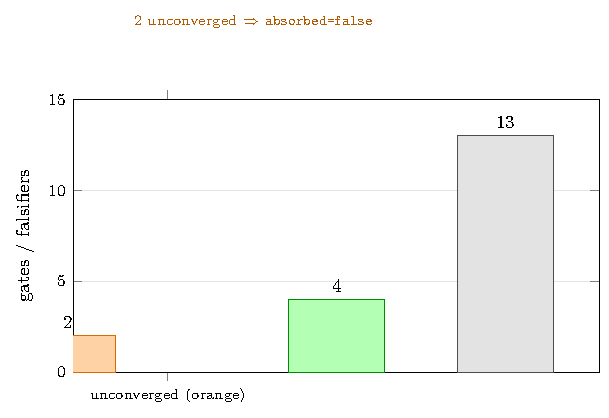
\includegraphics[width=0.84\linewidth]{figures/fig12_gate_status.pdf}
\caption{The non-wet-lab gate status: 2 \tierOrange\ unconverged (CFD,
$\circlearrowleft$), 4 \tierGreen\ closed (EM 6-coil, structural FEA,
thermal-cryo, F-ANTI-3), and 13 \tierWhite\ open (Stage-4--7 falsifiers,
empirical --- outside the non-wet-lab gate set). The two unconverged
\tierOrange\ gates are why \texttt{absorbed=false}; each has a named
pool/cloud closing path (@D~d7). The figure makes the verdict auditable:
a single unconverged gate is enough to hold the bit at \texttt{false}.}
\label{fig:gate-status}
\end{figure}

% -------------------------------------------------------------------------
\subsection{Breakthrough paths --- a wall is not an impossibility}
\label{app:gate-breakthrough}

Per @D~d2 we name a concrete breakthrough path for each remaining
blocker, never conceding impossibility. The CFD $C_d$/$L/D$ gate closes
with a pool \texttt{ubu} free dry-run followed by a vast.ai GPU DES; the
$\circlearrowleft$ 4-layer fixed point closes on a GPU pod running the
LC-2 coupling. Both are \emph{non-wet-lab} --- the same
external-solver/closed-form-anchor $\to$ heavy-body-solve pattern that
already closed the EM, stress, and thermal gates. On convergence the two
\tierOrange\ gates promote to \tierGreen\ and \texttt{absorbed} is
re-evaluated. Wet-lab measurement is the downstream confirmation, not the
gate (@D~d5).
